% To familiarize yourself with this template, the body contains
% some examples of its use.  Look them over.  Then you can
% run LaTeX on this file.  After you have LaTeXed this file then
% you can look over the result either by printing it out with
% dvips or using xdvi.
%

\documentclass[twoside,english]{article}
\setlength{\oddsidemargin}{0.25 in}
\setlength{\evensidemargin}{-0.25 in}
\setlength{\topmargin}{-0.6 in}
\setlength{\textwidth}{6.5 in}
\setlength{\textheight}{8.5 in}
\setlength{\headsep}{0.75 in}
\setlength{\parindent}{0 in}
\setlength{\parskip}{0.1 in}

%
% ADD PACKAGES here:
%

\usepackage{amsmath,amsfonts,graphicx,algorithm,caption}
\usepackage[noend]{algpseudocode}
\usepackage{hyperref}
\usepackage{natbib}
\usepackage[document]{ragged2e}
\usepackage{graphicx} %package to manage images
\usepackage{amsmath}
\usepackage{mathtools}
\usepackage{xcolor}

% The following commands set up the lecnum (lecture number)
% counter and make various numbering schemes work relative
% to the lecture number.
%
\newcounter{lecnum}
\renewcommand{\thepage}{\arabic{page}}
\renewcommand{\thesection}{\arabic{section}}
\renewcommand{\theequation}{\arabic{equation}}
\renewcommand{\thefigure}{\arabic{figure}}
\renewcommand{\thetable}{\arabic{table}}
\makeatletter
\def\BState{\State\hskip-\ALG@thistlm}
\makeatother
%
% The following macro is used to generate the header.
%
\newcommand{\lecture}[3]{
   \pagestyle{myheadings}
   \thispagestyle{plain}
   \newpage
   %\setcounter{lecnum}{#1}
   \setcounter{page}{1}
   \noindent
   \begin{center}
   \framebox{
      \vbox{\vspace{2mm}
    \hbox to 6.28in { {\bf IE 643: Deep Learning - Theory and Practice
		\hfill July-Dec 2026} }
       \vspace{4mm}
       \hbox to 6.28in { {\Large \hfill Project Report: #1  \hfill} }
       \vspace{2mm}
       \vspace{2mm}
       \hbox to 6.28in { {\it Team Name: #2 \hfill Team Members: #3} }
       %\vspace{2mm}}
       %\hbox to 6.28in { {\it Due Date: 01-August-2018} }
      \vspace{2mm}}
   }
   \end{center}
%   \markboth{Assignment #1: #2}{Assignment #1: #2}

   %{\bf Note}: {\it LaTeX template courtesy of UC Berkeley EECS dept.}

   %{\bf Disclaimer}: {\it These notes have not been subjected to the
   %usual scrutiny reserved for formal publications.  They may be distributed
   %outside this class only with the permission of the Instructor.}
   \vspace*{4mm}
}
%
% Convention for citations is authors' initials followed by the year.
% For example, to cite a paper by Leighton and Maggs you would type
% \cite{LM89}, and to cite a paper by Strassen you would type \cite{S69}.
% (To avoid bibliography problems, for now we redefine the \cite command.)
% Also commands that create a suitable format for the reference list.
% Teaching citation stub removed; natbib supplies actual citations.
\def\beginrefs{\begin{list}%
        {[\arabic{equation}]}{\usecounter{equation}
         \setlength{\leftmargin}{2.0truecm}\setlength{\labelsep}{0.4truecm}%
         \setlength{\labelwidth}{1.6truecm}}}
\def\endrefs{\end{list}}
\def\bibentry#1{\item[\hbox{[#1]}]}

%Use this command for a figure; it puts a figure in wherever you want it.
%usage: \fig{NUMBER}{SPACE-IN-INCHES}{CAPTION}
\newcommand{\fig}[3]{
			\vspace{#2}
			\begin{center}
			Figure #1:~#3
			\end{center}
	}
% Use these for theorems, lemmas, proofs, etc.
\newtheorem{theorem}{Theorem}[lecnum]
\newtheorem{lemma}[theorem]{Lemma}
\newtheorem{proposition}[theorem]{Proposition}
\newtheorem{claim}[theorem]{Claim}
\newtheorem{corollary}[theorem]{Corollary}
\newtheorem{definition}[theorem]{Definition}
\newenvironment{proof}{{\bf Proof:}}{\hfill\rule{2mm}{2mm}}

% **** IF YOU WANT TO DEFINE ADDITIONAL MACROS FOR YOURSELF, PUT THEM HERE:
\newcommand{\R}{\mathbb{R}}


\usepackage{booktabs,longtable,array,placeins}
\usepackage[T1]{fontenc}
\usepackage{lmodern}
\setlength{\emergencystretch}{2em}
\hypersetup{colorlinks=true,linkcolor=blue,citecolor=blue,urlcolor=blue,pdftitle={DeepGen - IE643 Intensive Assessment Report},pdfauthor={Ayush Patel; Rishik Yadav}}
\newcommand{\evidencefigure}[3]{\begin{figure}[htbp]\centering\includegraphics[width=#3\linewidth]{../../results/forecast_horizons/figures/#1}\caption{#2}\end{figure}}

\begin{document}
\lecture{Time-Series Domain Adaptation}{DeepGen}{23B0037, 23B2103}
\begin{center}
{\large\bfseries Lightweight multivariate forecasting with strictly observed-input adaptation}\\[2mm]
Ayush Patel (23B0037) \quad Rishik Yadav (23B2103)\\
Intensive assessment technical report \quad 20 October 2026
\end{center}

\begin{abstract}
This project studies forecasting under domain shift using three source--target pairs: hourly Shimla--Delhi weather, NSE IT--pharma financial features, and ETTh1--ETTh2 transformer measurements. The initial LiteTCN combines reversible normalization, temporal convolutions and a linear forecasting path. Its alignment/reconstruction adaptation is compared with MMD, CORAL, adversarial adaptation and labeled diagnostic references. Subsequent experiments test depth, linear and patch-based alternatives, strictly within-input self-supervision, source-guarded ensembles and several retained-TCN revisions. The original 24-hour weather/energy and five-trading-day finance tasks remain in the evaluation. A separate rolling next-hour task, added with explicit observation-refresh semantics, uses a small causal TCN, source-anchored local dynamics and a regime-dependent expert mixture calibrated on observed daily episodes. No original target forecasting labels are used in the strict adaptation or selection procedures. Final target temperature RMSE at one hour is 0.6530 degrees Celsius for climate and 0.9151 for energy, versus persistence 1.2692 and 1.3334. The corresponding source-only-to-adapted improvements are 3.84\% and 27.68\%; these must not be confused with changing forecast horizon. The strict finance ensemble improves standardized MSE approximately 1.60\% over input mean. Energy trough error and day-ahead peaks remain limitations. Saved models, stage-wise controls, plots, a CSV test interface and reproducibility checks accompany the report. The repeatedly inspected test periods are development evidence, not untouched confirmation.
\end{abstract}

\section{Introduction}
Forecasting functions learned in one location, sector or installation need not transfer unchanged to another. Differences include levels and variances, temporal dynamics, relationships between variables and the conditional distribution of future outcomes. The goal is to train a lightweight multivariate forecaster on a labeled source domain and adapt it using target histories while excluding the original target future labels.

Let $X\in\mathbb R^{L\times C}$ be an observed input and $Y\in\mathbb R^{H\times C}$ its original future. Source training has access to $(X_s,Y_s)$; strict target adaptation has access only to $X_t$. It may withhold a suffix \emph{inside that same input} for self-supervised prediction, but cannot use $Y_t$ or reconstruct it from neighboring windows. Evaluation uses actual target futures only after the relevant model choices are fixed.

The project pursues accuracy, adaptation benefit, retained source performance and computational cost. It also examines an important distinction between single-origin 24-hour forecasts and rolling next-hour forecasts. The latter receives new observations at every origin and is an additional operational task, not a new label for a day-ahead forecast. The course statement does not fix a horizon; the project retained the original benchmark while adding the shorter-horizon analysis.

This report follows the supplied course-template structure. Workflow and literature precede the methods, data and experiments. Results include negative controls and matched-horizon comparisons. Interface methodology, remaining limits and the novelty-assessment plan are included. Team contributions are based on the allocation supplied by the team: both members researched methods and carried out experiments; Ayush developed the dashboard/application, while Rishik prepared the report and presentation.

\section{Project Workflow}
\begin{itemize}
\item Acquire and preserve weather, financial and transformer data with distinct source/target domains; define variables and chronological splits.
\item Train source LiteTCN; compare alignment, reconstruction and anchoring adaptations against source-only and explicit labeled references.
\item Test additional TCN layers and simpler forecasters; use source validation and target-input pretexts rather than target futures for strict selection.
\item Develop channel-specific source-anchored predictors, guarded convex mixtures and a consistent shorter-context pretext.
\item Diagnose peak, trough, range and timing errors; retain LiteTCN through seasonal-folded, original-encoder residual, gradual-unfreezing and predicted-driver variants.
\item Test geometry-aware boosting for the original 24-hour task; add genuine one-hour TCN/dynamics models and observed-episode event calibration.
\item Freeze model choices, record metrics/plots and artifact hashes, then provide source/target CSV inference, comparison and downloads in a local interface.
\end{itemize}
The before-review baseline is the LiteTCN/CARE campaign documented in the prep assets. The later architecture, strict-pretext and peak-focused stages are distinguished below. The team should align that boundary with the exact prep presentation it delivered rather than infer individual authorship from file timestamps.

\section{Literature Survey}\label{sec:litsurvey}
Temporal convolutional sequence models motivate using dilation and parallel convolutional computation instead of a heavy recurrent architecture \citep{Bai18}. The project implements its own compact network; the initial strided encoder and the new causal one-hour encoder are different architectures. The original encoder can process the entire observed window without being a streaming-causal network inside that window.

RevIN removes and subsequently restores instance-level statistics to address distribution changes \citep{Kim22}. This inspires the original window normalization, but cannot by itself eliminate shifts in conditional forecasting dynamics. Domain-level training-period standardization and per-window reversible normalization are separate operations in the pipeline.

The linear forecasting study by Zeng et al. motivates comparing small decomposition/linear predictors seriously \citep{Zeng23}. The repository's DLinear-inspired implementation explicitly adds RevIN, so its numbers should not be presented as an exact paper reproduction. Its strong energy performance demonstrates why complexity must be justified empirically.

Deep CORAL aligns activation covariance \citep{Sun16}; domain-adversarial learning uses a domain discriminator with gradient reversal \citep{Ganin16}. These provide adaptation baselines rather than guarantees of forecasting improvement. In the saved campaign they can cause negative transfer. Kernel MMD measures a feature-distribution difference; even a lower discrepancy need not preserve the variable-specific information needed to forecast. The project's contribution is the integration and measured evaluation of these ideas with strict observed-input adaptation, guards and event calibration, not invention of the constituent TCN, normalization, ridge or boosting methods.

\section{Proposed Approach or Approaches}\label{sec:our_proj}
\subsection{Work before prep-presentation review: LiteTCN and CARE-DA}
The original hourly configuration has lookback 168, horizon 24 and seven channels. RevIN-normalized observations enter three strided Conv1d stages with GELU activations, followed by a latent projection and a direct horizon-by-channel head. A shared linear history-to-horizon path is added before reversing normalization. An auxiliary head reconstructs masked input observations. The stored hourly class has 381,606 parameters including reconstruction; the forecasting path without that auxiliary head has 229,902.

Source training minimizes forecast MSE plus optional masked reconstruction. The project-specific CARE-DA v1 recipe is
\begin{align}
L_{\mathrm{v1}}=L_{s}+L_{\mathrm{MMD}}+L_{\mathrm{CORAL}}+L_{\mathrm{recon},t}+0.01L_{\mathrm{anchor}}.
\end{align}
The source anchor penalizes movement from the source solution. DANN, CORAL-only, MMD-only and removal of alignment, self-supervision or anchoring are compared separately. Source labels remain permitted during adaptation.

CARE-DA v2 replaces reconstruction emphasis with forecast-consistent within-input prediction, noisy-view consistency and spectral feature alignment:
\begin{align}
L_{\mathrm{v2}}={}&L_s+L_{\mathrm{MMD},z}+0.5L_{\mathrm{MMD},h}+0.5L_{\mathrm{inner}}\nonumber\\
&+0.3L_{\mathrm{consistency}}+0.3L_{\mathrm{spectral}}+0.01L_{\mathrm{anchor}}.
\end{align}
Here $z$ denotes latent and $h$ pooled temporal features. The original three-seed campaign and the separately saved seed-0 v2 checkpoint are different artifacts. The original runner can calculate target-test error in diagnostic epoch snapshots; those values do not enter gradients or its fixed-budget checkpoint rule, but make the period visible during development.

\subsection{Work after prep-presentation review: capacity and forecasting-aligned adaptation}
Matched source-training controls test LiteTCN depths 3, 5 and 7, a custom patch/channel-mixing MLP, and a DLinear-inspired model. Extra layers do not consistently improve results. Source validation selects Patch MLP in each recorded seed/dataset of this sweep; target energy results nonetheless expose DLinear as a strong competitor. The custom MLP is not PatchTST.

A within-input forecasting task better matches deployment than masked reconstruction. For $L=168,H=24$, the predictor uses observed hours 1--144 and the self-supervised labels are hours 145--168. The original task's hours 169--192 remain excluded. A fixed-length network can left-pad from its own first prefix observation. A later shorter-context ridge branch instead uses a consistent 144-real-hour function, removing the padding mismatch for that branch.

Channel-specific ridge fits allow different normalizations and regularization per variable. Target fits combine within-input errors, labeled source replay and a coefficient anchor. A convex mixture retains source/adapted ridge, neural, DLinear and mean experts. Selection balances relative source-validation and target-input errors, constrains source degradation and includes the unchanged source solution as fallback. Broader exploratory history-reconstruction runs are retained as historical artifacts but excluded from the strict headline results.

\subsection{Retaining LiteTCN and investigating extremes}
LiteTCN v3 preserves hourly positions by seasonal folding, uses width-32 depthwise/pointwise dilated residual blocks, deterministic calendar features, a channel-specific seasonal skip and an attention-based direct decoder. Calendar/no-calendar and ordinary/shape-loss controls are recorded. It improves climate over the original saved model but is weaker for energy. A correction from observed recent residuals gives only small or mixed changes.

LiteTCN-R preserves the original source-trained encoder, initializes a linear skip from DLinear and fits a regularized residual head with source anchoring and zero-residual fallback. Gradual-unfreezing controls do not reliably beat the retained policy. A small coupled decoder then uses past history, clocks and \emph{predicted} future weather/load variables; actual future drivers are never supplied. Its retained-backbone composition yields effectively unchanged climate and a very small energy gain. These negative results are included rather than presenting the architecture as a universal improvement.

The 24-hour geometry-aware alternative uses CatBoost multi-output trees \citep{CatBoost}. Controls predict either the 24 temperature points directly or 16 DCT coefficients plus separately weighted maximum/minimum and circular peak/trough phase. Source/target-input validation chooses reconstruction/range/phase calibration and a 0/0.5/1 mixture with retained LiteTCN. Target adaptation adds trees using real prefixes and observed target tails, with source replay; source trees remain in the ensemble. Non-temperature variables remain exactly the backbone predictions.

\subsection{New next-hour source model and adaptation}
The new causal TCN has 8,903 parameters. From the last 48 observed rows it builds last-value-centered/scaled levels, differences and six clock features. Width-32 depthwise/pointwise residual blocks use dilations 1,2,4. A small head predicts a multivariate increment:
\begin{equation}
\widehat y_{t+1}=x_t+s(X)g_\theta(X),
\end{equation}
with a zero-initialized final layer, hence exact persistence at initialization. Future calendar features are analytically known, not future observations. The source loss combines global and key-temperature MSE; a turning control gives threefold key weight to genuine observed direction reversals.

Adaptation withholds the final observed hour of each target X, replays source examples and anchors relative layer weights:
\begin{equation}
L_{\mathrm{adapt}}=L_{\mathrm{inner},t}+0.5L_{s,\mathrm{replay}}+0.001L_{\mathrm{relative\ anchor}}.
\end{equation}
The local-dynamics branch fits next-hour changes from normalized trajectories, past multivariate statistics and clocks. Target normal equations include source replay and a coefficient anchor. A guarded first-stage mixture combines neural, dynamics and persistence experts.

\subsection{Final event-aligned regime calibration}
The final system contains five outer experts: source/adapted versions of the new one-hour hybrid, source/adapted first-hour outputs of the earlier strict hybrid, and persistence. For variable $c$ and an observed regime $r$, weights satisfy $w_{crj}\geq0$ and $\sum_jw_{crj}=1$. Source-only routes cannot use adapted experts.

Four causal regimes are defined from the last three observations and past 48-hour scale: ordinary motion, approaching a peak, approaching a trough and flat/observed reversal. If $d_t=x_t-x_{t-1}$ and $a_t=d_t-d_{t-1}$, the heuristic estimated turning time is $-d_t/a_t$, subject to slope/acceleration signs and a three-step interval. Actual future extrema never enter this regime rule.

Calibration constructs successive one-hour forecasts over 24 steps entirely inside a validation X. At each inner origin, only the preceding prefix is visible. Let $e_i=\widehat y_i-y_i$, and let $i_+,i_-$ be the actual observed maximum/minimum indices in that calibration episode. The per-variable event loss is
\begin{align}
L_{\mathrm{event}}={}&\frac1{24}\sum_i e_i^2+2\frac{e_{i_+}^2+e_{i_-}^2}{2}\nonumber\\
&+0.1\frac1{23}\sum_{i=1}^{23}\big[(\widehat y_{i+1}-\widehat y_i)-(y_{i+1}-y_i)\big]^2.
\end{align}
Actual extrema define \emph{loss weights on observed calibration labels}, not inference features. The target calibration objective is
\begin{align}
J(w)={}&\tfrac12\frac{L_{\mathrm{event},s}(w)}{L_{\mathrm{event},s}(w_s)}+
\tfrac12\frac{L_{\mathrm{event},tX}(w)}{L_{\mathrm{event},tX}(w_s)}+0.001\|w-w_s\|_2^2.
\end{align}
Frozen-expert weights are fitted by constrained SLSQP. Source point error may increase by at most 10\% over the source-calibrated reference, target-input point error by at most 5\%, and regimes need at least 64 source/target examples before adapting. Failed/ineligible solutions revert to the source mixture. Source outer calibration itself has a 5\% point guard against its feasible initial source expert. These are measured calibration constraints, not bounds on every future event.

\section{Data set Details}\label{sec:data}
\begin{longtable}{@{}p{.12\textwidth}p{.23\textwidth}p{.17\textwidth}p{.18\textwidth}p{.195\textwidth}@{}}
\caption{Configured benchmark pairs. Splits are chronological train/validation/test.}\\\toprule
Benchmark&Source to target&Rows per domain&Variables / cadence&Lookback / horizon / split\\\midrule\endhead
Climate&Shimla to Delhi&35,064&7 / hourly&168 / 24; 70/10/20\%\\
Finance&Five IT to five pharma stocks&16,610 (3,322 per stock)&4 / trading day&60 / 5; 70/10/20\%\\
Energy&ETTh1 to ETTh2&17,420&7 / hourly&168 / 24; 60/20/20\%\\\bottomrule
\end{longtable}
Weather covers 1 January 2021 through 31 December 2024, downloaded from the Open-Meteo archive with Asia/Kolkata timestamps \citep{OpenMeteo}. Variables are temperature, relative humidity, dew point, surface pressure, wind speed, cloud cover and shortwave radiation. Coordinates are Shimla (31.1048,77.1734) and Delhi (28.6139,77.2090). The request does not pin one archive model; these should not be presented as direct station measurements or a uniquely pinned ERA5 product.

ETT covers 1 July 2016 through 26 June 2018 19:00 \citep{ETT}. The columns HUFL, HULL, MUFL, MULL, LUFL, LULL and OT are forecast. OT is transformer \emph{oil} temperature, not ambient weather temperature or total electricity consumption. Future actual load variables are not forecasting inputs.

Financial downloads use adjusted OHLCV via yfinance \citep{Finance}. Source stocks are TCS, INFY, WIPRO, HCLTECH and TECHM; target stocks are SUNPHARMA, DRREDDY, CIPLA, DIVISLAB and LUPIN. Processed dates span 3 January 2012--27 June 2025. Features are $100\log(C_t/C_{t-1})$, $100\log(H_t/L_t)$, $100\log(O_t/C_{t-1})$ and $\log(1+V_t)$. The primary finance metric is the log high--low range, not closing-price or index RMSE. Separate stocks remain separate series; windows never cross company boundaries.

Each domain uses statistics from its raw training period; finance pools its five training series. The cached convention includes final training-period rows not appearing in a complete training X, but excludes validation/test rows. Validation/test segments receive preceding historical context. Training stride is two for climate and one otherwise; evaluated origins advance one step in the original benchmark. The weather downloader interpolates missing values in both directions before saving; this is offline preparation, not an online causal imputation guarantee. Processed feature columns contain no missing values. Exact data hashes accompany the runs.

The H=1 benchmark scores only the first future value at the same original test origins: 6,990 climate and 3,461 energy. It does not add the final 23 possible H=1 origins. Nearby windows/forecasts are correlated; their count must not be treated as an independent sample size.

\section{Experiments}\label{sec:exp}
The original source budget is 20 epochs with AdamW learning rate 0.001, batch 256 and cosine decay; original adaptation uses a fixed ten-epoch campaign. The later architecture sweep uses 15 source and up to eight adaptation epochs. LiteTCN v3 uses 36 sampled rounds and ten adaptation rounds, at most 4,096 sampled windows per round. The new one-hour TCN uses 28 sampled source rounds, AdamW 0.001, weight decay 0.0001, batch 256 and cosine decay; its adapter uses 12 sampled rounds at 0.0002. A sampled round is not a full-dataset epoch.

The tree controls use up to 400 source trees at 0.06 and up to 400 added target-input trees at 0.04, depth 4, 32 histogram borders and leaf L2 10. Stage counts, geometry decoding and mixture strength are selected on source/target-X proxies with a 5\% source key-MSE guard. An added-tree removal control retains the selected backbone/postprocessing/mixture while removing the new target stages.

For the final observed-episode calibration, the first $L$ validation origins are purged and episode windows sampled every 25 origins so their 24-hour label tails do not overlap. Prefix padding uses only that prefix's first observation. Source and target datasets and seeds 0,1,2 are fitted before the recorded test inference for each latest experiment. The app deploys seed 0; table means are not a three-seed deployment ensemble.

Experiments ran on CPU PyTorch 2.6.0, Python 3.13.2, AMD Ryzen 5 5600H (6 physical cores, 12 logical processors). Latest neural training uses two threads. The numerical environment is recorded in \texttt{requirements-experiments.txt}; CatBoost is 1.2.10. Hash audits identify code, initial experts, data and frozen checkpoints. Earlier test periods and additional climate periods were already inspected, so no untouched confirmation is claimed. Within-run freezing does not erase project-level development reuse.

\subsection{Metrics and baseline contract}
Standardized multivariate MSE/MAE average over variables and horizon steps. Key-variable RMSE is inverse-transformed to degrees Celsius for climate/energy and log high--low range units for finance. MSE is not accuracy in percent and is not comparable across different datasets as a common physical quantity. Persistence repeats the last observation; seasonal naive repeats the recent season (24 for hourly tasks, 1 for finance); input mean repeats the input average.

The original window-scaled MAE denominator is computed inside each input; later \texttt{MASE\_train} uses fixed per-variable training-period seasonal differences. The two columns are not interchangeable. H=1 still uses the configured training seasonal scale. Peak/trough MAE is measured at the \emph{actual} extrema's time index, distinct from max/min-value bias. Timing compares argmax indices; ramp error compares first differences. H=1 event metrics group successive forecasts into non-overlapping 24-hour episodes and omit the final incomplete episode. Main point metrics retain the full original-origin cohort.

\subsection{Negative controls and excluded interpretations}
Deeper TCNs, reconstruction-heavy alignment, source-backbone coupled decoders and late unfreezing are not consistently successful. Broader cross-window history pilots are excluded from strict headline results. Target-only and supervised fine-tuned fits are labeled references, not eligible label-free deployments or mathematical upper bounds. The source-subset fitting sanity check is a training diagnostic: on 64 climate source windows the new TCN fitting RMSE falls from 1.7603 to 0.5035 after 128 updates, but that is not held-out accuracy. A source-only climate ridge comparison improves validation RMSE 1.7734 to 1.7243 when past weather is added; it does not establish causal effects or target transfer.

\section{Results}\label{sec:results}
\subsection{Original adaptation and depth experiments}
{\footnotesize
\setlength{\tabcolsep}{3pt}
\renewcommand{\arraystretch}{1.17}
\begin{longtable}{@{}p{0.5278\textwidth}p{0.1911\textwidth}p{0.1911\textwidth}@{}}
\caption{Original source/adaptation campaign, target MSE, three seeds.}\label{tab:original_table}\\
\toprule
Dataset & Original method (3 seeds) & MSE \\
\midrule\endfirsthead
Dataset & Original method (3 seeds) & MSE \\
\midrule\endhead
\midrule\multicolumn{3}{r}{Continued on next page}\\\endfoot
\bottomrule\endlastfoot
climate & source\_\allowbreak{}only & 0.2537 \\
climate & care & 0.2446 \\
climate & mmd & 0.2338 \\
climate & coral & 0.2717 \\
climate & dann & 0.2676 \\
energy & source\_\allowbreak{}only & 0.1728 \\
energy & care & 0.1671 \\
energy & mmd & 0.1652 \\
energy & coral & 0.1925 \\
energy & dann & 0.2171 \\
finance & source\_\allowbreak{}only & 0.5611 \\
finance & care & 0.5616 \\
finance & mmd & 0.5584 \\
finance & coral & 0.5726 \\
finance & dann & 0.5724 \\
\end{longtable}
}

{\footnotesize
\setlength{\tabcolsep}{3pt}
\renewcommand{\arraystretch}{1.17}
\begin{longtable}{@{}p{0.1092\textwidth}p{0.4550\textwidth}p{0.1729\textwidth}p{0.1729\textwidth}@{}}
\caption{Original saved CARE-DA v2 comparison: fixed seed 0, not a three-seed v2 mean.}\label{tab:v2_table}\\
\toprule
Dataset & Saved seed-0 method & MSE & Key RMSE \\
\midrule\endfirsthead
Dataset & Saved seed-0 method & MSE & Key RMSE \\
\midrule\endhead
\midrule\multicolumn{4}{r}{Continued on next page}\\\endfoot
\bottomrule\endlastfoot
climate & source\_\allowbreak{}only & 0.2512 & 1.7591 \\
climate & care\_\allowbreak{}v1 & 0.2449 & 1.6765 \\
climate & care\_\allowbreak{}v2 & 0.2357 & 1.4739 \\
energy & source\_\allowbreak{}only & 0.1691 & 4.6086 \\
energy & care\_\allowbreak{}v1 & 0.1632 & 4.4421 \\
energy & care\_\allowbreak{}v2 & 0.1559 & 4.1827 \\
finance & source\_\allowbreak{}only & 0.5622 & 1.0855 \\
finance & care\_\allowbreak{}v1 & 0.5634 & 1.0881 \\
finance & care\_\allowbreak{}v2 & 0.5520 & 1.0732 \\
\end{longtable}
}

{\footnotesize
\setlength{\tabcolsep}{3pt}
\renewcommand{\arraystretch}{1.17}
\begin{longtable}{@{}p{0.1092\textwidth}p{0.4550\textwidth}p{0.1729\textwidth}p{0.1729\textwidth}@{}}
\caption{Matched source-training architecture sweep evaluated on the target, three seeds. No target Y is used to choose the source architecture.}\label{tab:depth_table}\\
\toprule
Dataset & Source-trained candidate & Target MSE & Target key RMSE \\
\midrule\endfirsthead
Dataset & Source-trained candidate & Target MSE & Target key RMSE \\
\midrule\endhead
\midrule\multicolumn{4}{r}{Continued on next page}\\\endfoot
\bottomrule\endlastfoot
climate & tcn3 & 0.2552 & 1.6372 \\
climate & tcn5 & 0.2583 & 1.6168 \\
climate & tcn7 & 0.2615 & 1.6783 \\
climate & patch\_\allowbreak{}mlp & 0.2261 & 1.3490 \\
climate & dlinear & 0.2288 & 1.3578 \\
energy & tcn3 & 0.1751 & 4.6012 \\
energy & tcn5 & 0.1747 & 4.6306 \\
energy & tcn7 & 0.1758 & 4.6655 \\
energy & patch\_\allowbreak{}mlp & 0.1594 & 4.2545 \\
energy & dlinear & 0.1446 & 4.0982 \\
finance & tcn3 & 0.5607 & 1.0824 \\
finance & tcn5 & 0.5614 & 1.0824 \\
finance & tcn7 & 0.5610 & 1.0817 \\
finance & patch\_\allowbreak{}mlp & 0.5502 & 1.0735 \\
finance & dlinear & 0.5498 & 1.0630 \\
\end{longtable}
}

The original CARE result is mixed, especially finance; MMD alone can outperform full CARE. Extra TCN layers do not consistently improve forecasting. The full original ablation and labeled references are provided in the appendix rather than selecting only favorable comparisons.

\subsection{Original-horizon strict policies and retained-TCN follow-ups}
{\footnotesize
\setlength{\tabcolsep}{3pt}
\renewcommand{\arraystretch}{1.17}
\begin{longtable}{@{}p{0.5278\textwidth}p{0.1911\textwidth}p{0.1911\textwidth}@{}}
\caption{Climate, single-origin H=24: target development results. Key RMSE in degrees Celsius.}\label{tab:long_climate}\\
\toprule
Model / policy & Standardized MSE & Key-variable RMSE \\
\midrule\endfirsthead
Model / policy & Standardized MSE & Key-variable RMSE \\
\midrule\endhead
\midrule\multicolumn{3}{r}{Continued on next page}\\\endfoot
\bottomrule\endlastfoot
Original CARE-DA v2, fixed seed 0 & 0.2357 & 1.4739 \\
First validation-selected adapted model & 0.2225 & 1.3342 \\
Strict input-only ensemble & 0.2174 & 1.3234 \\
Shorter-context strict ensemble & 0.2160 & 1.2836 \\
LiteTCN v3 adapted & 0.2206 & 1.3284 \\
LiteTCN v3 + observed residual calibration & 0.2207 & 1.3226 \\
LiteTCN-R adapted & 0.2276 & 1.3781 \\
Gradual-unfreezing follow-up & 0.2284 & 1.3856 \\
Retained TCN + predicted-driver decoder & 0.2206 & 1.3293 \\
Retained TCN + geometry-aware boosting & 0.2205 & 1.3136 \\
seasonal\_\allowbreak{}naive & 0.3513 & 1.5532 \\
persistence & 0.7557 & 5.4498 \\
input\_\allowbreak{}mean & 0.5234 & 4.1348 \\
\end{longtable}
}

{\footnotesize
\setlength{\tabcolsep}{3pt}
\renewcommand{\arraystretch}{1.17}
\begin{longtable}{@{}p{0.5278\textwidth}p{0.1911\textwidth}p{0.1911\textwidth}@{}}
\caption{Energy, single-origin H=24: target development results. Key RMSE is oil-temperature degrees Celsius.}\label{tab:long_energy}\\
\toprule
Model / policy & Standardized MSE & Key-variable RMSE \\
\midrule\endfirsthead
Model / policy & Standardized MSE & Key-variable RMSE \\
\midrule\endhead
\midrule\multicolumn{3}{r}{Continued on next page}\\\endfoot
\bottomrule\endlastfoot
Original CARE-DA v2, fixed seed 0 & 0.1559 & 4.1827 \\
First validation-selected adapted model & 0.1532 & 4.2142 \\
DLinear source-only (all seeds) & 0.1446 & 4.0982 \\
Guarded DLinear family policy & 0.1448 & 4.0749 \\
Strict input-only ensemble & 0.1456 & 3.9762 \\
Shorter-context strict ensemble & 0.1456 & 3.9995 \\
LiteTCN v3 adapted & 0.1678 & 4.1789 \\
LiteTCN v3 + observed residual calibration & 0.1642 & 4.1912 \\
LiteTCN-R adapted & 0.1462 & 4.0991 \\
Gradual-unfreezing follow-up & 0.1468 & 4.0773 \\
Retained TCN + predicted-driver decoder & 0.1461 & 4.0835 \\
Retained TCN + geometry-aware boosting & 0.1456 & 4.0168 \\
seasonal\_\allowbreak{}naive & 0.2246 & 4.7699 \\
persistence & 0.2572 & 6.4598 \\
input\_\allowbreak{}mean & 0.2522 & 6.7445 \\
\end{longtable}
}

{\footnotesize
\setlength{\tabcolsep}{3pt}
\renewcommand{\arraystretch}{1.17}
\begin{longtable}{@{}p{0.5278\textwidth}p{0.1911\textwidth}p{0.1911\textwidth}@{}}
\caption{Finance, H=5 trading days: target development results. Key RMSE is 100 log(high/low), not price RMSE.}\label{tab:long_finance}\\
\toprule
Model / policy & Standardized MSE & Key-variable RMSE \\
\midrule\endfirsthead
Model / policy & Standardized MSE & Key-variable RMSE \\
\midrule\endhead
\midrule\multicolumn{3}{r}{Continued on next page}\\\endfoot
\bottomrule\endlastfoot
Original CARE-DA v2, fixed seed 0 & 0.5520 & 1.0732 \\
First validation-selected adapted model & 0.5475 & 1.0712 \\
Strict input-only ensemble & 0.5373 & 1.0658 \\
Shorter-context strict ensemble & 0.5373 & 1.0657 \\
seasonal\_\allowbreak{}naive & 1.0240 & 1.4027 \\
persistence & 1.0240 & 1.4027 \\
input\_\allowbreak{}mean & 0.5460 & 1.0731 \\
\end{longtable}
}

The shorter-context climate ensemble remains a strong H=24 policy at MSE 0.2160 and temperature RMSE 1.2836. Energy raw source DLinear MSE 0.1446 is slightly better on the development test than its guarded family policy 0.1448; that test observation does not authorize a retrospectively reselected deployment policy. The strict energy mixture has lower oil-temperature RMSE 3.9762 despite slightly higher global MSE, and the ridge-only adapted control reaches approximately 3.9539. Consequently no universal best model is claimed.

The geometry boost improves retained-TCN temperature RMSE from 1.3284 to 1.3136 (climate) and 4.0991 to 4.0168 (energy), only 1.11\% and 2.01\%. It does not surpass all earlier references. The retained-TCN coupled decoder's changes are still smaller and mixed. Finance strict MSE 0.5373 versus input mean 0.5460 is a 1.60\% reduction; its gain over the strong strict source-only ensemble MSE approximately 0.5380 is only 0.14\%. Neither number establishes a profitable trading strategy.
\evidencefigure{climate_single_origin_24h.png}{Climate: fixed first/middle/last single-origin 24-hour examples. The forecasts do not receive actual observations inside the horizon.}{.98}
\evidencefigure{energy_single_origin_24h.png}{Energy oil temperature: the same single-origin comparison. Day-ahead amplitude and timing errors remain visible.}{.98}
\FloatBarrier

\subsection{Rolling next-hour results and source retention}
{\footnotesize
\setlength{\tabcolsep}{3pt}
\renewcommand{\arraystretch}{1.17}
\begin{longtable}{@{}p{0.1092\textwidth}p{0.1820\textwidth}p{0.1729\textwidth}p{0.1820\textwidth}p{0.1319\textwidth}p{0.1319\textwidth}@{}}
\caption{Final peak-calibrated H=1 hybrid, target temperature RMSE, three-seed means. Comparisons share the same horizon.}\label{tab:rolling_headline}\\
\toprule
Dataset & Source-only RMSE (degC) & Adapted RMSE (degC) & Persistence RMSE (degC) & Adaptation reduction (\%) & Reduction vs persistence (\%) \\
\midrule\endfirsthead
Dataset & Source-only RMSE (degC) & Adapted RMSE (degC) & Persistence RMSE (degC) & Adaptation reduction (\%) & Reduction vs persistence (\%) \\
\midrule\endhead
\midrule\multicolumn{6}{r}{Continued on next page}\\\endfoot
\bottomrule\endlastfoot
climate & 0.6791 & 0.6530 & 1.2692 & 3.8439 & 48.5486 \\
energy & 1.2653 & 0.9151 & 1.3334 & 27.6755 & 31.3690 \\
\end{longtable}
}

{\footnotesize
\setlength{\tabcolsep}{3pt}
\renewcommand{\arraystretch}{1.17}
\begin{longtable}{@{}p{0.1092\textwidth}p{0.4550\textwidth}p{0.1729\textwidth}p{0.1729\textwidth}@{}}
\caption{Matched next-hour comparisons. The original checkpoint is fixed seed 0; other fitted families average three seeds.}\label{tab:rolling_comparison}\\
\toprule
Dataset & Same 1-hour task & MSE & Temperature RMSE (degC) \\
\midrule\endfirsthead
Dataset & Same 1-hour task & MSE & Temperature RMSE (degC) \\
\midrule\endhead
\midrule\multicolumn{4}{r}{Continued on next page}\\\endfoot
\bottomrule\endlastfoot
climate & Earlier hybrid, first-hour output & 0.0819 & 0.6540 \\
climate & Next-hour LiteTCN & 0.0798 & 0.7445 \\
climate & Next-hour LiteTCN + local dynamics & 0.0776 & 0.6926 \\
climate & Original LiteTCN first-hour (fixed seed 0) & 0.1205 & 1.0089 \\
climate & Peak-calibrated next-hour hybrid & 0.0781 & 0.6530 \\
energy & Earlier hybrid, first-hour output & 0.0590 & 0.9462 \\
energy & Next-hour LiteTCN & 0.0714 & 1.1002 \\
energy & Next-hour LiteTCN + local dynamics & 0.0647 & 0.8970 \\
energy & Original LiteTCN first-hour (fixed seed 0) & 0.0765 & 2.0938 \\
energy & Peak-calibrated next-hour hybrid & 0.0606 & 0.9151 \\
\end{longtable}
}

{\footnotesize
\setlength{\tabcolsep}{3pt}
\renewcommand{\arraystretch}{1.17}
\begin{longtable}{@{}p{0.2912\textwidth}p{0.1547\textwidth}p{0.1547\textwidth}p{0.1547\textwidth}p{0.1547\textwidth}@{}}
\caption{Both evaluated domains for final H=1 source-only and adapted models, three-seed means.}\label{tab:source_retention}\\
\toprule
Dataset & Evaluated domain & Model & MSE & Temperature RMSE \\
\midrule\endfirsthead
Dataset & Evaluated domain & Model & MSE & Temperature RMSE \\
\midrule\endhead
\midrule\multicolumn{5}{r}{Continued on next page}\\\endfoot
\bottomrule\endlastfoot
climate & source & adapted\_\allowbreak{}model & 0.0868 & 0.8700 \\
climate & source & source\_\allowbreak{}model & 0.0843 & 0.8710 \\
climate & target & adapted\_\allowbreak{}model & 0.0781 & 0.6530 \\
climate & target & source\_\allowbreak{}model & 0.0809 & 0.6791 \\
energy & source & adapted\_\allowbreak{}model & 0.1328 & 0.6356 \\
energy & source & source\_\allowbreak{}model & 0.1382 & 0.6371 \\
energy & target & adapted\_\allowbreak{}model & 0.0606 & 0.9151 \\
energy & target & source\_\allowbreak{}model & 0.0649 & 1.2653 \\
\end{longtable}
}

At fixed H=1, adaptation reduces final source-only temperature RMSE by 3.84\% climate and 27.68\% energy. Reductions versus persistence are 48.55\% and 31.37\%, including source learning, expert choices and adaptation. Lower H=1 errors versus H=24 are partly caused by a different information/task setting and cannot be presented as adaptation-only gains.

The earlier climate first-hour hybrid already has RMSE 0.6540, nearly the final 0.6530. The first new next-hour energy hybrid has lower temperature RMSE 0.8970 than the final peak calibration 0.9151, while the earlier energy reference has lower global MSE. These tradeoffs are retained rather than imposing a test-selected winner policy. Source-domain test errors are also reported; source-validation guards do not guarantee every source test score improves.
\evidencefigure{rolling_next_hour_overview.png}{Rolling H=1 overview, deployment seed 0. Every point is predicted from preceding observations, with model weights frozen. First 96 origins, not error-selected examples.}{.98}
\evidencefigure{climate_rolling_next_hour.png}{Climate rolling forecasts at fixed first, middle and last 96-hour segments, with the same observation-refresh rule for every compared model.}{.98}
\evidencefigure{energy_rolling_next_hour.png}{Energy rolling forecasts at fixed first, middle and last 96-hour segments. New observations reveal events as they occur; this is not a day-ahead curve.}{.98}
\FloatBarrier

\subsection{Peak/trough behavior, adaptation curves and ablations}
{\footnotesize
\setlength{\tabcolsep}{3pt}
\renewcommand{\arraystretch}{1.17}
\begin{longtable}{@{}p{0.2912\textwidth}p{0.1547\textwidth}p{0.1547\textwidth}p{0.1547\textwidth}p{0.1547\textwidth}@{}}
\caption{Errors over non-overlapping 24-hour episodes of successive H=1 forecasts; the last incomplete episode is omitted.}\label{tab:peak_table}\\
\toprule
Dataset & Model & Peak MAE (degC) & Trough MAE (degC) & Peak timing error (hours) \\
\midrule\endfirsthead
Dataset & Model & Peak MAE (degC) & Trough MAE (degC) & Peak timing error (hours) \\
\midrule\endhead
\midrule\multicolumn{5}{r}{Continued on next page}\\\endfoot
\bottomrule\endlastfoot
climate & Earlier hybrid, first-hour output & 0.2622 & 0.5620 & 0.7354 \\
climate & Next-hour TCN/baselines & 0.4354 & 0.6612 & 0.7457 \\
climate & Persistence & 0.3646 & 0.6168 & 1.2955 \\
climate & Next-hour hybrid & 0.4472 & 0.6545 & 0.7079 \\
climate & Peak-calibrated next-hour hybrid & 0.2810 & 0.5514 & 0.7342 \\
energy & Earlier hybrid, first-hour output & 0.9120 & 0.7987 & 1.7245 \\
energy & Next-hour TCN/baselines & 0.9599 & 0.8420 & 2.0301 \\
energy & Persistence & 0.9628 & 0.4761 & 2.1528 \\
energy & Next-hour hybrid & 0.8588 & 0.7342 & 1.5556 \\
energy & Peak-calibrated next-hour hybrid & 0.8477 & 0.6650 & 1.4213 \\
\end{longtable}
}

Compared with the first new next-hour hybrid, final calibration reduces climate peak/trough MAE from 0.4472/0.6545 to 0.2810/0.5514 and energy from 0.8588/0.7342 to 0.8477/0.6650. Energy peak gain is small. Persistence still has lower energy trough MAE 0.4761, and final adaptation worsens trough MAE relative to its source-only calibration even while improving overall RMSE. This is a specific remaining negative-transfer result.

Under squared loss the optimal point predictor is a conditional mean; uncertainty in peak time can flatten that mean. Unknown future weather/load changes, transfer mismatch and pretext/architecture mismatch also contribute. The controls do not isolate a unique cause. Sharpening an inaccurate or mistimed curve is not sufficient evidence of improvement.
\evidencefigure{climate_next_hour_adaptation.png}{Climate neural adaptation: source-validation, withheld target-input error and selection proxy. These are not target-test selection curves or final-hybrid learning curves.}{.95}
\evidencefigure{energy_next_hour_adaptation.png}{Energy neural adaptation, with the same source/observed-input selection semantics.}{.95}
\evidencefigure{climate_peak_calibration.png}{Final climate seed-0 calibration on episodes entirely inside observed histories. Source retention is a bounded tradeoff, not guaranteed improvement.}{.95}
\evidencefigure{energy_peak_calibration.png}{Final energy observed-episode calibration. The original target forecasting Y tensors do not enter this fit.}{.95}
{\footnotesize
\setlength{\tabcolsep}{3pt}
\renewcommand{\arraystretch}{1.17}
\begin{longtable}{@{}p{0.5278\textwidth}p{0.1911\textwidth}p{0.1911\textwidth}@{}}
\caption{H=24 added-tree control with backbone, decoder and mixture held fixed; this is not a separately reselected source-only policy.}\label{tab:boost_ablation}\\
\toprule
Dataset & Added-tree control & Temperature RMSE \\
\midrule\endfirsthead
Dataset & Added-tree control & Temperature RMSE \\
\midrule\endhead
\midrule\multicolumn{3}{r}{Continued on next page}\\\endfoot
\bottomrule\endlastfoot
climate & New target trees removed & 1.4067 \\
climate & New target-input trees retained & 1.3136 \\
energy & New target trees removed & 4.1986 \\
energy & New target-input trees retained & 4.0168 \\
\end{longtable}
}

Removing new target trees isolates their contribution for the chosen H=24 configuration, but the retained backbone may already be adapted. Final event calibration versus the first hybrid is a whole-system comparison: experts and regime structure also change, so it is not a clean event-loss-only ablation. Identical-expert point/event and regime/no-regime controls remain future work.
\FloatBarrier

\subsection{Efficiency and verification}
{\footnotesize
\setlength{\tabcolsep}{3pt}
\renewcommand{\arraystretch}{1.17}
\begin{longtable}{@{}p{0.1092\textwidth}p{0.1820\textwidth}p{0.1729\textwidth}p{0.1820\textwidth}p{0.1319\textwidth}p{0.1319\textwidth}@{}}
\caption{Deployment CPU efficiency. KB includes active native trees; neural counts exclude native tree leaves and coefficient buffers.}\label{tab:efficiency}\\
\toprule
Dataset & Family & Neural parameters & Stored tensor values & Deployed KB & CPU ms / single forecast \\
\midrule\endfirsthead
Dataset & Family & Neural parameters & Stored tensor values & Deployed KB & CPU ms / single forecast \\
\midrule\endhead
\midrule\multicolumn{6}{r}{Continued on next page}\\\endfoot
\bottomrule\endlastfoot
climate & next\_\allowbreak{}hour & 8903 & 8903 & 44.5078 & 2.4648 \\
climate & next\_\allowbreak{}hour\_\allowbreak{}hybrid & 17806 & 19339 & 97.8545 & 4.7463 \\
climate & event\_\allowbreak{}boost & 44399 & 44399 & 2575.9395 & 5.7487 \\
climate & peak\_\allowbreak{}next\_\allowbreak{}hour & 110840 & 171901 & 711.8262 & 9.4504 \\
energy & next\_\allowbreak{}hour & 8903 & 8903 & 44.5078 & 2.1180 \\
energy & next\_\allowbreak{}hour\_\allowbreak{}hybrid & 17806 & 19339 & 97.8545 & 6.7387 \\
energy & event\_\allowbreak{}boost & 229902 & 229902 & 2412.3496 & 3.4754 \\
energy & peak\_\allowbreak{}next\_\allowbreak{}hour & 110840 & 179965 & 743.3262 & 11.7343 \\
\end{longtable}
}

The new standalone TCN is approximately 44.5 KB. The final hybrid has 110,840 neural parameters and approximately 712/743 KB serialized tensors for climate/energy, including coefficient buffers. Single-forecast CPU latency is approximately 9.45/11.73 ms on this machine. The benchmark uses batch 1, five warmups, 30 repeats and one PyTorch thread; active native tree prediction uses two threads. These are measurements for this configuration, not claims against every competing model.

The complete current suite passes 46 tests, covering 76 archived research-interface combinations and all 36 submission-interface combinations. The model-experiment stage alone previously recorded 40 tests. The new assessment-interface/backend tests additionally check future-row isolation, exact exported actuals, duplicate headers, hourly gaps, input-only forecasting, horizon mismatch and all 36 submitted dataset/domain/horizon/model combinations (ten primary dataset/domain/horizon settings). The latest complete verification log accompanies the package and is the source for its final check count. Artifact audits cover eight latest family/dataset combinations, validate hashes and selection arithmetic, and recompute complete deployment seed-0 source/target MSE. These checks establish implementation properties, not statistical optimality. Three-seed RMSE SD is approximately 0.0038/0.0140 degrees Celsius for the final climate/energy model; it is not uncertainty over future years.

\subsection{Interface design and use}
The assessment interface is a local Streamlit application with a forecast studio, benchmark dashboard and method/downloads page. Dataset, horizon and model are explicit choices. Source versus target selects the corresponding saved scaler and checkpoint; this is not automatic unknown-domain recognition. It offers only strict supported workflows, while the earlier experiment explorer is preserved separately.

The user uploads one chronological multivariate CSV or uses bundled source/target examples. Header and value checks reject duplicates, missing/nonfinite variables, multiple series and invalid dates; hourly models require consecutive timestamps. Financial OHLCV can be converted to the configured features. At least L usable rows are needed for forecasting, and L+H for a complete actual future. The plotted input stops at the chosen origin; actual future data is used only for scoring. Models remain frozen during upload inference and historical evaluation.

Window metrics are labeled separately from saved benchmark means and file-wide evaluation. Historical evaluation starts longer forecasts every H rows without internal updates and refreshes H=1 inputs hourly. The user chooses the maximum latest origins, which are stated in the output. Source/adapted, persistence, seasonal and input-mean errors share the same truth and horizon. Forecasts, evaluated actuals and metrics can be downloaded. With input-only data the app forecasts after the last row and shows no fabricated error score. Finance displayed future dates follow weekdays rather than an exchange-holiday calendar.

A separate HTML dashboard embeds its charts and Plotly for offline use, with explicit dataset and horizon filters. It reports both source and target evidence and event metrics. It is a results viewer, not a replacement for the CSV inference app. Run the latter with \texttt{python -m streamlit run app/app.py}; the preserved research explorer is \texttt{app/research.py}.
\begin{figure}[htbp]\centering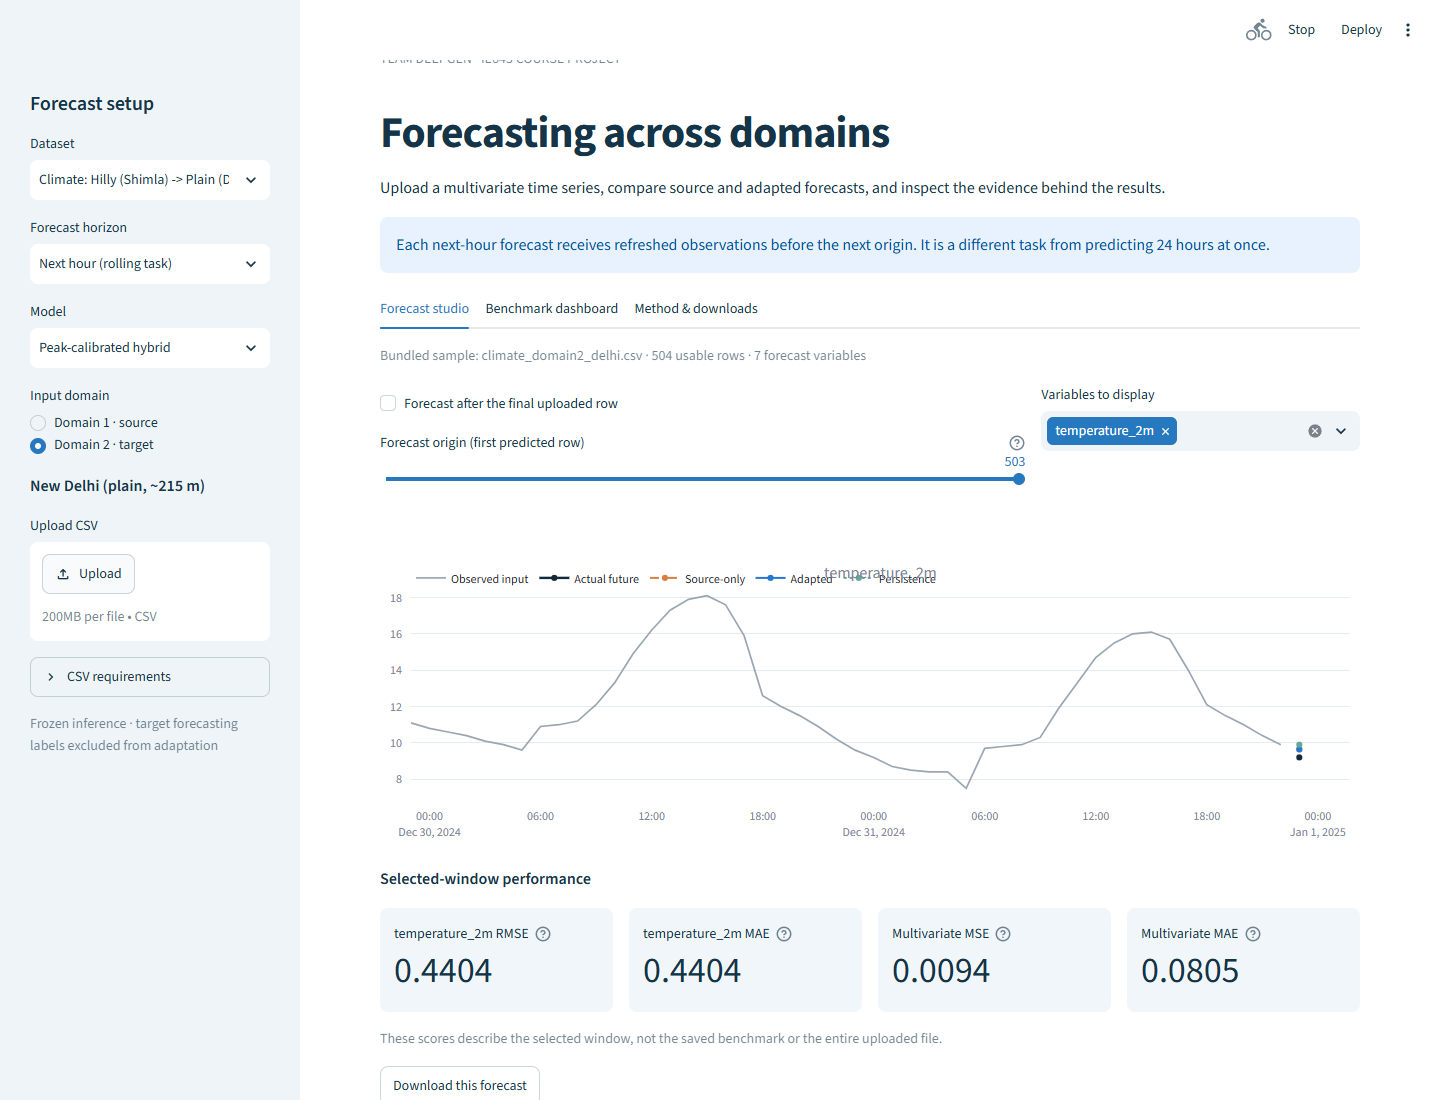
\includegraphics[width=.98\linewidth]{figures/app_studio.png}\caption{Assessment interface with dataset, horizon, source/target setup, historical observations, actual future and frozen forecast overlays. The displayed window score is separate from benchmark averages.}\end{figure}
\begin{figure}[htbp]\centering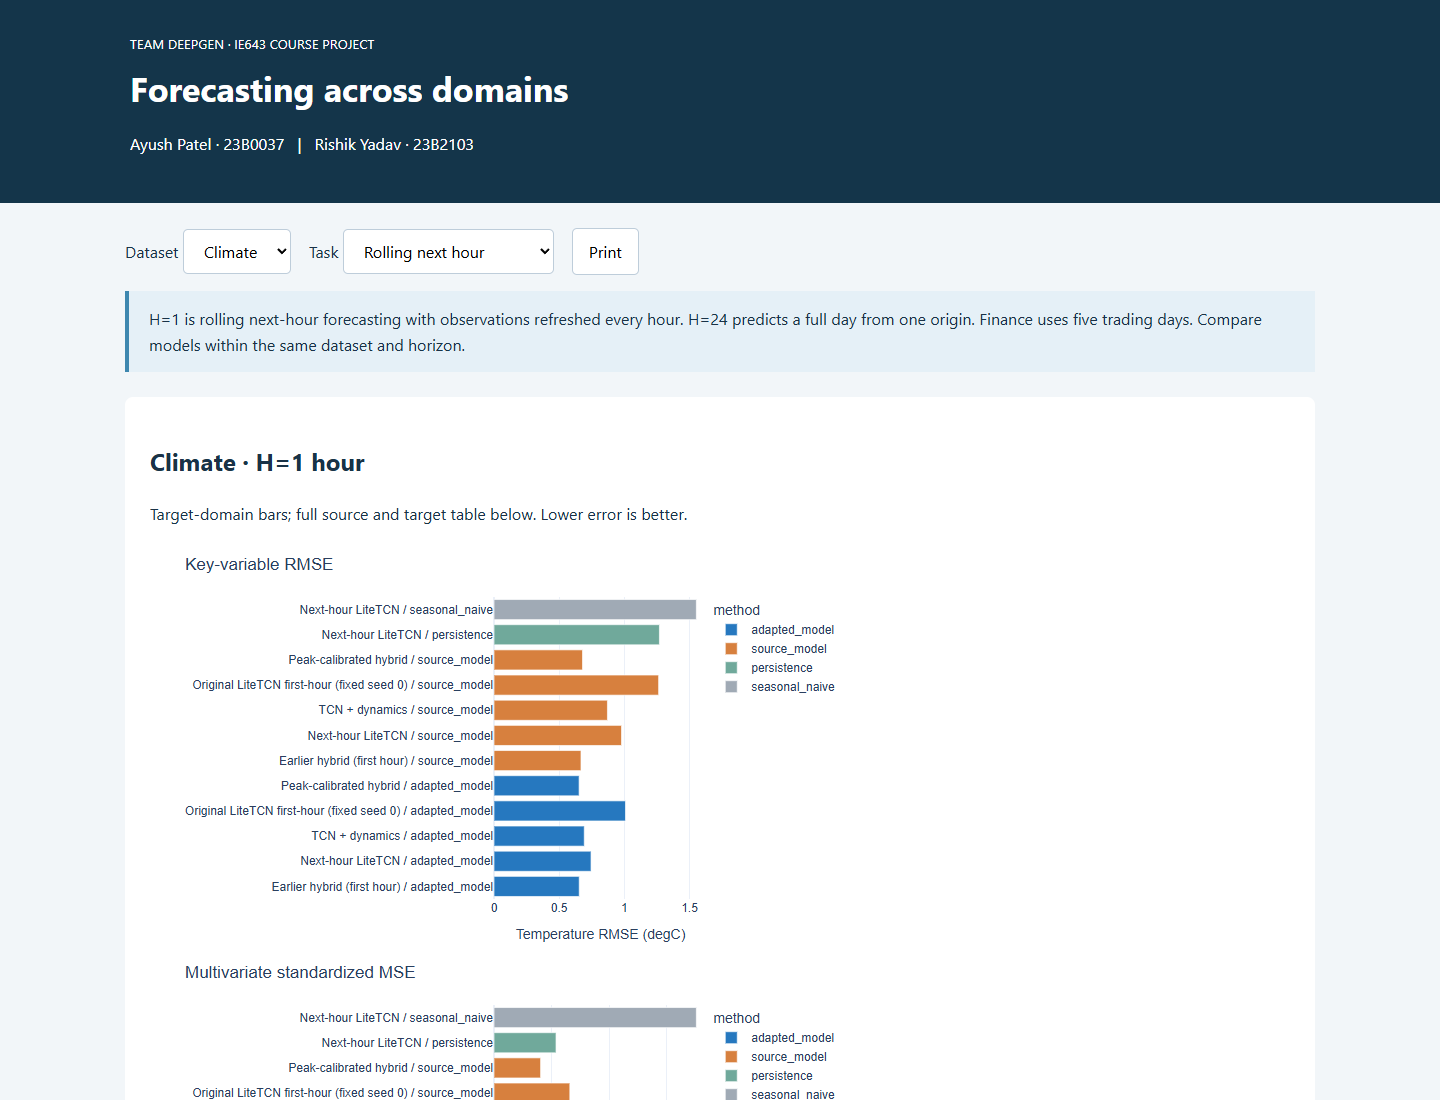
\includegraphics[width=.98\linewidth]{figures/offline_dashboard.png}\caption{Offline dashboard with explicit dataset and task filters. Embedded charts and source/target tables do not require a running server.}\end{figure}
\FloatBarrier

\section{Plan for Novelty Assessment}\label{sec:Plan for Novelty Assessment}
A useful next stage first locks an untouched chronological period. With identical expert outputs and data, compare point-only versus event loss, then regime-dependent versus constant calibration. Use time-block uncertainty rather than treating overlapping origins as independent. Investigate energy trough failure cases and robust/probabilistic objectives. Test external driver forecasts only when they are actually available at the forecast origin. Finally evaluate distillation/compression of the hybrid into a smaller standalone TCN. These are proposed experiments, not completed outcomes or publication-level novelty claims.

\section{Conclusion}\label{sec:conclusion}
The project implements source and adapted forecasting across three domain pairs, retains lightweight TCN models through multiple controlled revisions, and improves on strong baselines using strictly observed-input adaptation. Deeper layers alone do not solve the original errors. Source-guarded forecasting pretexts and hybrid predictors are stronger in these experiments; event calibration improves specific rolling peak/trough metrics with measurable ordinary-error tradeoffs. The final H=1 temperature RMSE is 0.6530/0.9151, but energy troughs, original H=24 extremes and reused-test generalization remain limitations. All claims specify dataset, horizon, metric and comparison basis. Code, saved models, data/selection provenance, result plots and reviewer-facing inference accompany the report. The configured GitHub remote is listed in the references \citep{Code}; local package inclusion does not imply that all changes have been pushed remotely.

\clearpage
\bibliographystyle{plainnat}
\bibliography{references}
\clearpage
\appendix
\section{Complete recorded control tables}
The following tables preserve original ablations and the subsequent recorded methods, including failures. Target-only and fine-tuned references explicitly use target labels and are excluded from strict deployment claims. Original-screen rows can have one seed while selected policies use three; consult the associated selection/manifest files rather than interpreting every row as a new independent trial.
{\footnotesize
\setlength{\tabcolsep}{3pt}
\renewcommand{\arraystretch}{1.17}
\begin{longtable}{@{}p{0.1092\textwidth}p{0.4550\textwidth}p{0.1729\textwidth}p{0.1729\textwidth}@{}}
\caption{Complete original campaign including negative ablations and explicitly label-using reference fits.}\label{tab:original_complete}\\
\toprule
Dataset & Original campaign method & MSE & Key RMSE \\
\midrule\endfirsthead
Dataset & Original campaign method & MSE & Key RMSE \\
\midrule\endhead
\midrule\multicolumn{4}{r}{Continued on next page}\\\endfoot
\bottomrule\endlastfoot
climate & care & 0.2446 & 1.6488 \\
climate & care\_\allowbreak{}noalign & 0.2684 & 1.9929 \\
climate & care\_\allowbreak{}noanchor & 0.2441 & 1.5638 \\
climate & care\_\allowbreak{}nossl & 0.2339 & 1.4202 \\
climate & coral & 0.2717 & 1.6901 \\
climate & dann & 0.2676 & 1.7178 \\
climate & mmd & 0.2338 & 1.3874 \\
climate & oracle\_\allowbreak{}finetune & 0.2321 & 1.4112 \\
climate & seasonal\_\allowbreak{}naive & 0.3513 & 1.5532 \\
climate & source\_\allowbreak{}only & 0.2537 & 1.7678 \\
climate & target\_\allowbreak{}only & 0.2402 & 1.4334 \\
energy & care & 0.1671 & 4.5246 \\
energy & care\_\allowbreak{}noalign & 0.1805 & 4.7850 \\
energy & care\_\allowbreak{}noanchor & 0.1726 & 4.6952 \\
energy & care\_\allowbreak{}nossl & 0.1617 & 4.3519 \\
energy & coral & 0.1925 & 5.2325 \\
energy & dann & 0.2171 & 5.6488 \\
energy & mmd & 0.1652 & 4.4881 \\
energy & oracle\_\allowbreak{}finetune & 0.1676 & 4.2628 \\
energy & seasonal\_\allowbreak{}naive & 0.2246 & 4.7699 \\
energy & source\_\allowbreak{}only & 0.1728 & 4.6542 \\
energy & target\_\allowbreak{}only & 0.1774 & 4.5388 \\
finance & care & 0.5616 & 1.0844 \\
finance & care\_\allowbreak{}noalign & 0.5643 & 1.0878 \\
finance & care\_\allowbreak{}noanchor & 0.5641 & 1.0873 \\
finance & care\_\allowbreak{}nossl & 0.5580 & 1.0798 \\
finance & coral & 0.5726 & 1.1003 \\
finance & dann & 0.5724 & 1.1000 \\
finance & mmd & 0.5584 & 1.0816 \\
finance & oracle\_\allowbreak{}finetune & 0.5478 & 1.0670 \\
finance & seasonal\_\allowbreak{}naive & 1.0240 & 1.4027 \\
finance & source\_\allowbreak{}only & 0.5611 & 1.0830 \\
finance & target\_\allowbreak{}only & 0.5507 & 1.0725 \\
\end{longtable}
}

{\footnotesize
\setlength{\tabcolsep}{3pt}
\renewcommand{\arraystretch}{1.17}
\begin{longtable}{@{}p{0.2912\textwidth}p{0.1547\textwidth}p{0.1547\textwidth}p{0.1547\textwidth}p{0.1547\textwidth}@{}}
\caption{Additional recorded controls. Family names indicate experiment stage; screen controls can be seed 0, whereas selected policies average three seeds. H=1 families begin at next\_\allowbreak{}hour.}\label{tab:additional_controls}\\
\toprule
Recorded family / method & climate MSE & climate key\_\allowbreak{}RMSE & energy MSE & energy key\_\allowbreak{}RMSE \\
\midrule\endfirsthead
Recorded family / method & climate MSE & climate key\_\allowbreak{}RMSE & energy MSE & energy key\_\allowbreak{}RMSE \\
\midrule\endhead
\midrule\multicolumn{5}{r}{Continued on next page}\\\endfoot
\bottomrule\endlastfoot
peak\_\allowbreak{}litetcn / input\_\allowbreak{}mse & 0.2188 & 1.3280 & 0.1672 & 4.1729 \\
peak\_\allowbreak{}litetcn / input\_\allowbreak{}shape & 0.2215 & 1.3288 & 0.1684 & 4.2001 \\
peak\_\allowbreak{}litetcn / screen\_\allowbreak{}clock\_\allowbreak{}mse & 0.2359 & 1.4201 & 0.1859 & 4.7128 \\
peak\_\allowbreak{}litetcn / screen\_\allowbreak{}clock\_\allowbreak{}shape & 0.2429 & 1.4188 & 0.1866 & 4.6265 \\
peak\_\allowbreak{}litetcn / screen\_\allowbreak{}no\_\allowbreak{}clock\_\allowbreak{}mse & 0.2339 & 1.4029 & 0.1823 & 4.3960 \\
peak\_\allowbreak{}litetcn / selected\_\allowbreak{}adapted & 0.2206 & 1.3284 & 0.1678 & 4.1789 \\
peak\_\allowbreak{}litetcn / source\_\allowbreak{}only & 0.2393 & 1.4327 & 0.1788 & 4.6285 \\
peak\_\allowbreak{}calibrated / local\_\allowbreak{}adapted & 0.2207 & 1.3226 & 0.1642 & 4.1912 \\
peak\_\allowbreak{}calibrated / local\_\allowbreak{}source & 0.2371 & 1.4205 & 0.1725 & 4.6104 \\
peak\_\allowbreak{}calibrated / raw\_\allowbreak{}adapted & 0.2206 & 1.3284 & 0.1678 & 4.1789 \\
peak\_\allowbreak{}calibrated / raw\_\allowbreak{}source & 0.2393 & 1.4327 & 0.1788 & 4.6285 \\
residual\_\allowbreak{}litetcn / adapted\_\allowbreak{}residual\_\allowbreak{}tcn & 0.2276 & 1.3781 & 0.1462 & 4.0991 \\
residual\_\allowbreak{}litetcn / linear\_\allowbreak{}skip\_\allowbreak{}only & 0.2288 & 1.3578 & 0.1446 & 4.0982 \\
residual\_\allowbreak{}litetcn / source\_\allowbreak{}residual\_\allowbreak{}tcn & 0.2298 & 1.4319 & 0.1466 & 4.0858 \\
progressive\_\allowbreak{}litetcn / adapted\_\allowbreak{}model & 0.2284 & 1.3856 & 0.1468 & 4.0773 \\
progressive\_\allowbreak{}litetcn / head\_\allowbreak{}only & 0.2299 & 1.4329 & 0.1466 & 4.0858 \\
progressive\_\allowbreak{}litetcn / progressive & 0.2299 & 1.4329 & 0.1466 & 4.0858 \\
progressive\_\allowbreak{}litetcn / source\_\allowbreak{}model & 0.2299 & 1.4329 & 0.1466 & 4.0858 \\
coupled\_\allowbreak{}litetcn / adapted\_\allowbreak{}model & 0.2391 & 1.4075 & 0.1466 & 4.0894 \\
coupled\_\allowbreak{}litetcn / coupled & 0.2393 & 1.4401 & 0.1483 & 4.2917 \\
coupled\_\allowbreak{}litetcn / source\_\allowbreak{}model & 0.2393 & 1.4401 & 0.1468 & 4.1139 \\
coupled\_\allowbreak{}litetcn / temperature\_\allowbreak{}only & 0.2393 & 1.4351 & 0.1468 & 4.1139 \\
coupled\_\allowbreak{}transfer / adapted\_\allowbreak{}backbone\_\allowbreak{}only & 0.2206 & 1.3284 & 0.1462 & 4.0991 \\
coupled\_\allowbreak{}transfer / adapted\_\allowbreak{}model & 0.2206 & 1.3293 & 0.1461 & 4.0835 \\
coupled\_\allowbreak{}transfer / source\_\allowbreak{}decoder\_\allowbreak{}on\_\allowbreak{}adapted\_\allowbreak{}backbone & 0.2207 & 1.3368 & 0.1462 & 4.0933 \\
coupled\_\allowbreak{}transfer / source\_\allowbreak{}model & 0.2393 & 1.4401 & 0.1468 & 4.1139 \\
event\_\allowbreak{}boost / adapted\_\allowbreak{}model & 0.2205 & 1.3136 & 0.1456 & 4.0168 \\
event\_\allowbreak{}boost / retained\_\allowbreak{}backbone & 0.2206 & 1.3284 & 0.1462 & 4.0991 \\
event\_\allowbreak{}boost / source\_\allowbreak{}model & 0.2395 & 1.4685 & 0.1474 & 4.1914 \\
next\_\allowbreak{}hour / adapted\_\allowbreak{}model & 0.0798 & 0.7445 & 0.0714 & 1.1002 \\
next\_\allowbreak{}hour / source\_\allowbreak{}model & 0.0901 & 0.9784 & 0.0802 & 1.3500 \\
next\_\allowbreak{}hour\_\allowbreak{}hybrid / adapted\_\allowbreak{}model & 0.0776 & 0.6926 & 0.0647 & 0.8970 \\
next\_\allowbreak{}hour\_\allowbreak{}hybrid / source\_\allowbreak{}model & 0.0852 & 0.8704 & 0.0682 & 1.3945 \\
peak\_\allowbreak{}next\_\allowbreak{}hour / adapted\_\allowbreak{}model & 0.0781 & 0.6530 & 0.0606 & 0.9151 \\
peak\_\allowbreak{}next\_\allowbreak{}hour / source\_\allowbreak{}model & 0.0809 & 0.6791 & 0.0649 & 1.2653 \\
\end{longtable}
}


\section{Artifacts and reproducibility}
The source code covers collection/preprocessing (\texttt{config.py}, \texttt{data\_download.py}, \texttt{data.py}), original models/losses (\texttt{model.py}, \texttt{train.py}, \texttt{losses.py}), strict/shorter-context ensembles, TCN revisions, 24-hour boosting and the final \texttt{nowcast\_tcn.py}, \texttt{nowcast\_hybrid.py}, \texttt{peak\_nowcast.py} training modules. Inference and assessment evaluation are in \texttt{inference.py}, \texttt{submission.py} and \texttt{app/submission\_app.py}. The final source/adapted checkpoints reside under \texttt{models/peak\_next\_hour/}; finance remains under \texttt{models/strict\_refined/finance/}. Original-horizon strict and TCN/boost artifacts are retained.

Exact numerical evidence is in \texttt{results/forecast\_horizons/}, per-family CSVs, calibration JSONs and selection-freeze manifests. \texttt{numerical\_sources.json} records hashes used for report table production. \texttt{template\_provenance.json} identifies the supplied template and minimal technical changes. Earlier reports and PPTs are preserved rather than overwritten. A staged package manifest identifies included files; source raw API download files are distinguished from processed data. Reproduction of the latest stages requires the earlier expert checkpoints named by their manifests, not only the most recent training command.

\begin{verbatim}
pip install -r requirements-experiments.txt
python -m unittest discover -s tests -v
python -m src.check_horizon_models
python -m streamlit run app/app.py
\end{verbatim}
The offline dashboard and study guide require no running server. Documentation/report builders are separate from model fitting; regenerating a report does not train or change a model. Team dataset approval, final narrative review, video recording, remote synchronization and actual submission access are administrative tasks separate from model correctness. The final report should be reviewed and explained by both authors in accordance with the course's authorship instructions.
\end{document}
